\documentclass[12pt, letterpaper]{article}
% must use this pkg for displaying imgs
\usepackage{graphicx}
\usepackage{amsmath}
\usepackage{multirow,array}
\usepackage{blindtext}
\usepackage{etoolbox}
\usepackage[a4paper, total={6in, 9in}]{geometry}
\graphicspath{ {../../imgs/} }
% pkg for links
\usepackage{hyperref}
% for codeblocks highlighting
\usepackage{listings}
\lstset{language=C}


\makeatletter
\patchcmd{\raggedright}{\parindent\z@}{}{}{}
\makeatother

\begin{document}


\newcommand{\paperauthor}{Akiel Aries}
\newcommand{\papersupervisor}{Prof. Sareh Assiri}
\newcommand{\paperuniversity}{Northern Arizona University}

\newcommand{\papertitle}{Analyzing and Reporting on}
\newcommand{\paperminortitle}{Stuxnet}
\newcommand{\papermajorheading}{Cybersecurity}
\newcommand{\paperminorheading}{CYB 410 - Software Security}

\newcommand{\HRule}{\rule{\linewidth}{0.5mm}} % Defines a new command for the horizontal lines, change thickness here

\center % Center everything on the page

%----------------------------------------------------------------------------------------
%	HEADING SECTIONS
%----------------------------------------------------------------------------------------

\textsc{\LARGE \paperuniversity}\\[1.0cm] % Name of your university/college
\textsc{\Large \papermajorheading}\\[0.2cm] % Major heading such as course name
\textsc{\large \paperminorheading}\\[0.75cm] % Minor heading such as course title

%----------------------------------------------------------------------------------------
%	TITLE SECTION
%----------------------------------------------------------------------------------------

\HRule \\[0.4cm]
{ \huge \bfseries \papertitle}\\[0.05cm] % Title of your document
{ \huge \paperminortitle}\\[0.025cm] % Title of your document
\HRule \\[3.5cm]

\begin{center}
	\makebox[1.0\textwidth]{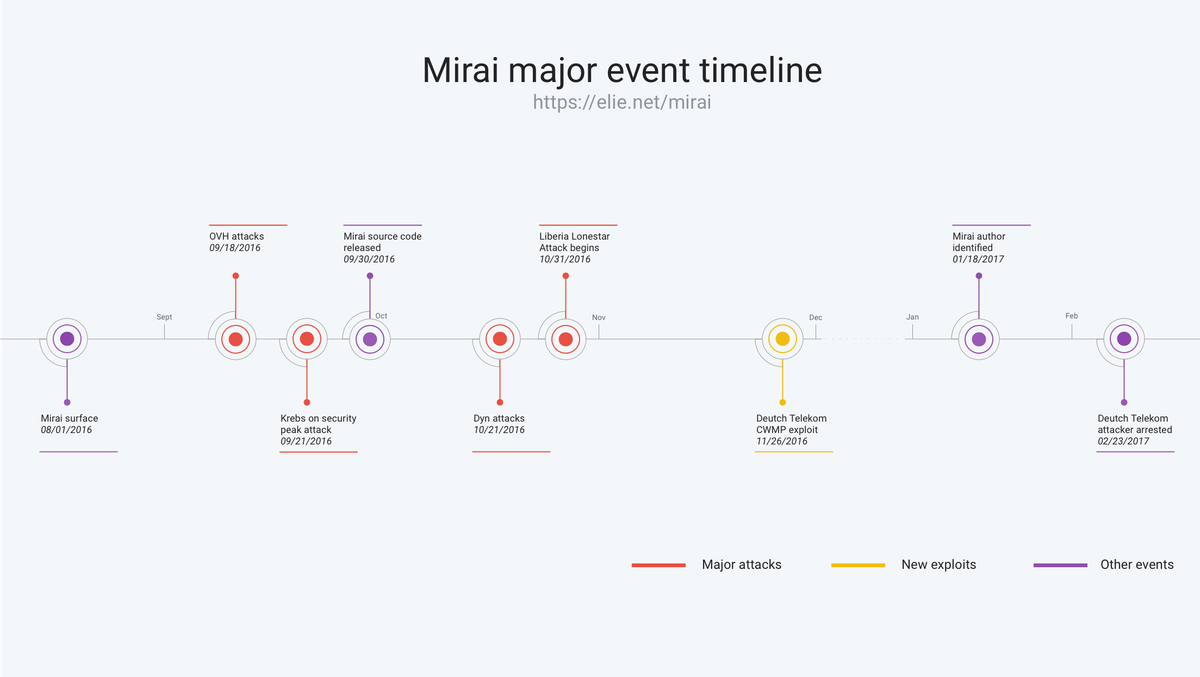
\includegraphics[width=1.0\textwidth]{mirai-major-events-timeline.png}}
\end{center}


\vfill % Fill the rest of the page with whitespace
%----------------------------------------------------------------------------------------
%	AUTHOR SECTION
%--------------------------------------------------------------------------------------

\begin{minipage}{0.4\textwidth}
	\begin{flushleft} \large
	\emph{Author:}\\
	\paperauthor
	\end{flushleft}
	\end{minipage}
	~
	\begin{minipage}{0.4\textwidth}
	\begin{flushright} \large
	\emph{Professor:} \\
	\papersupervisor
	\end{flushright}
\end{minipage}\\[1cm]

%----------------------------------------------------------------------------------------
%	DATE SECTION
%----------------------------------------------------------------------------------------
{\large \today}\\ % Date, change the \today to a set date if you want to be precise

\newpage

\begin{sloppypar}


% classification img
%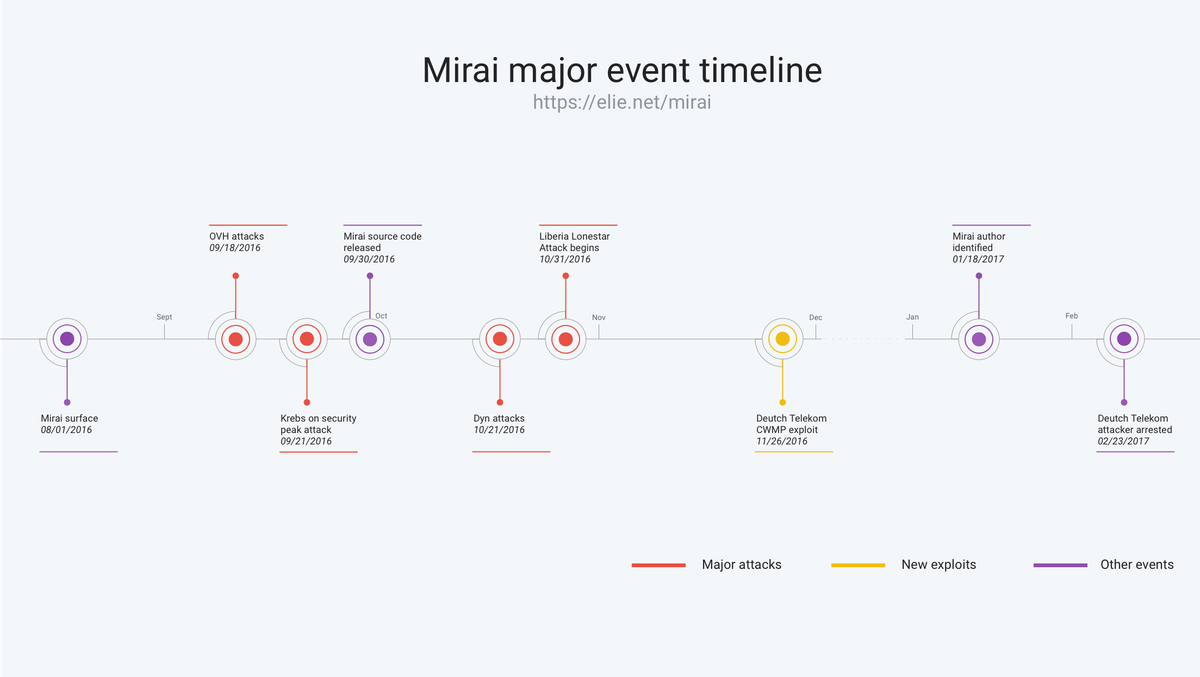
\includegraphics[scale=0.3]{mirai-major-events-timeline.png}
\begin{flushleft}
\section{Overview}
\begin{center}
{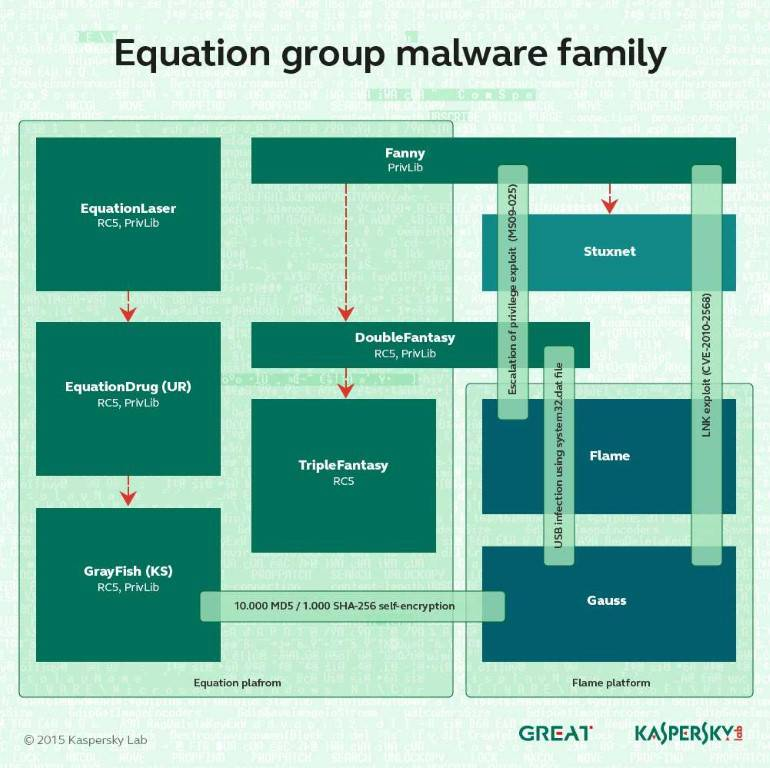
\includegraphics[width=0.9\textwidth]{equation_group_family.jpg}}
\end{center}

PLCs (Programmable Logic Controller)

%\newpage

\section{Source Code}


%\newpage

\section*{Scale}


\section*{Execution}


\section*{Reproducible Example}


\section*{Static Analysis/Debugging}


\section*{Fuzzing with AFL}


\section*{Final Notes}

\end{flushleft}
\end{sloppypar}
\end{document}
